\chapter{Experiments on Domain Mixture Scenario with Domain Separation Networks} \label{ch:experiment}
In the last section, we covered the scenarios in focus of this thesis: the complete domain mixture scenario. This is the situation in which the source domain is consisted of multiple domains mixed together and, as the name implies, all the domains have complete representations of all the classes. However, the domains are only complete but none of the involving domain is completely supervised, i.e., only samples of some classes represented in a single domain come with labels. Only through mixing those domains together do we achieve a source domain with complete supervised representations of the classes. The goal of the domain adaptation in this case is to train a network using this mixed source domain to perform a classification task on samples in these domains that it only has seen unsupervisedly without labels. In our experiment, we use the setup with only two domains involved and the mixture of them creates the source and target domain. First, the datasets used will be introduced before necessary definitions and notations of the experiments are summarized

\paragraph*{Datasets} For our experiments, we use the MNIST and the MNIST-M dataset. The MNIST \cite{mnist} dataset contains grayscale pictures of handwritten digits from 0 to 9 with 60,000 training images and 10,000 test images. The MNIST-M \cite{mnist-m} is created by inverting colors of the MNIST images by cropped images from the Berkeley Segmentation Data Set and Benchmarks 500 (BSDS500) \cite{bsds500}. It contains 59,001 training images and 9,001 test images. Due to the color modification, these two datasets represent two different domains. In this section, we will refer to the MNIST dataset and the MNIST-M dataset as $S$ and $M$ respectively to conform with \cite{domainMixture}. Samples from these datasets are shown in Figure \ref{fig:mnistmnistm}

\begin{figure}[tbh]
  \centering
  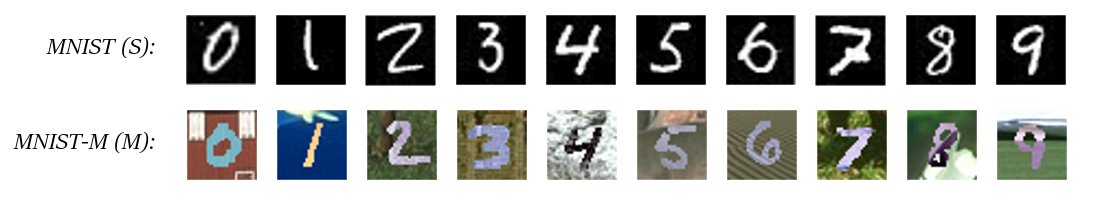
\includegraphics[width=0.8\textwidth]{abbildungen/mnistmnistmText.png}
  \caption{MNIST and MNIST-M: MNIST contains grayscale images while MNIST-M contains color images. They represent different domains.}
  \label{fig:mnistmnistm}
\end{figure}

\section*{Notations and Definitions}
\paragraph*{Source Domain $\mathcal{D}_S$} The source domain is the mixture of S and M with $m$ classes of supervised samples. For the complete supervised training samples, we use $m \in \{5, 6, 7, 8, 9\}$. More details will be discussed further in the next section.
\paragraph*{Target Domain $\mathcal{D}_T$} The target domain is also the mixture of S and M which is involved only unsupervisedly in the training and is used to perform the evaluation of the trained model.
\paragraph*{Training Parameters} According to the total loss function in \eqref{eq:lossesDSN} mentioned in section \ref{ch:dsn}, the DSN has the parameters: $\alpha$ controlling the reconstruction loss, $\beta$ controlling the difference loss and $\gamma$ controlling the similarity loss as can be seen again in equation \ref{eq:lossesDSN}. 
	\begin{equation}
			\mathcal{L} = \mathcal{L}_{Task} + \alpha \mathcal{L}_{recon} + \beta \mathcal{L}_{difference} + \gamma \mathcal{L}_{similarity}  \tag{\ref{eq:lossesDSN}}
	\end{equation}
The authors of DSN used $\alpha \in [0.01, 0.15]$, $\beta \in [0.05, 0.075]$ and $\gamma \in [0.25, 0.3]$. From the original implementation in Github, the learning rate $\lambda = 0.011724$ and $\gamma = 0.251175$ were given, which are also used in the experiments. For other parameters, we use $\alpha = 0.01$ and $\beta = 0.05$ if the corresponding losses should be activated. Since the goal of the experiments is not to exactly compare the performance of the model absolutely to other experiments, but rather to compare the performances of the network between different setups, these chosen values should suffice for our purpose. 
\paragraph*{Outputs} The classifier of the DSN makes a prediction about the class the input most likely belongs to. This predicted label is denoted $\hat{y}$ and the real label of the input is $y$.  \\

\section{Experimental Setups} \label{sec:exSetups}
The goal for the experiments is to observe the effects of the missing class samples and the mixture of the domain in the learning process. The standard scenario of domain adaptation is training a model on a complete domain to be able to adapt to another domain which we also use as our baseline. Then, in comparison to this standard case, the experiments are done with the mixed source and target domain $\mathcal{D}_S$ and $\mathcal{D}_T$ by combining $S$ and $M$ so that $\mathcal{D}_S$ includes supervised samples of all the 10 classes as mentioned above. Then the number of the supervised classed $m$ is altered to allow the influence of the overlapping between two domains on the training to be observed. Furthermore, the effect of different loss function combinations are evaluated. 
The network is trained for different number of steps depending on the complexity of the network - how many losses of the network were activated. If there are more constraints and more training data involved, we let the network train longer. In every step, the batch gradient descent algorithm is used with 32 samples in a batch randomly chosen from the domain mixtures. The mixtures are created by mixing images from $S$ and $M$ and shuffling them together. As mentioned above, the model used the same hyperparameters in all setups, if the losses are activated, and was trained with the same initial learning rate. We also use an exponential learning rate decay of 0.95 every 20,000 steps to ease the convergence and prevent overfitting, these values were also used in the original implementation. Equation \eqref{eq:expDecay} shows the exponential learning rate decay with the decay factor $d$, the global step $s_{glob}$, the overall step taken in the training, and the decay step $s_{decay}$, the number of steps taken before the learning rate decay should be activated.

	\begin{equation} \label{eq:expDecay}
			\lambda = \lambda d^{\frac{s_{glob}}{s_{decay}}}
	\end{equation}

Then, the network is also trained with different loss functions combinations. Table \ref{tb:lossCombinations} shows the combinations experimented.  
\begin{table}[h!]
\begin{center}
\begin{tabular}{l|lll}
Activated Parameters & $\alpha$ & $\beta$ & $\gamma$ \\ \hline
noDA                 & 0        & 0       & 0        \\
DSN'                 & 0.01     & 0.05    & 0.251175 \\
recon                & 0.01     & 0       & 0        \\
diff                 & 0        & 0.05    & 0        \\
sim                  & 0        & 0       & 0.251175 \\
nosim                & 0.01     & 0.05    & 0        \\
nodiff               & 0.01     & 0       & 0.251175 \\
norec                & 0        & 0.05    & 0.251175
\end{tabular}
\caption{Various loss combinations of the DSN with our hyperparameters: The DSN is trained without domain adaptation i.e. no losses activated, with all losses and all combinations of the losses.}
\label{tb:lossCombinations}
\end{center}
\end{table}

Then, for simplicity, the networks related to the experiments will be referred to as in Table \ref{tb:networkNames}.

\begin{table}[h!]
\begin{center}
\begin{tabular}{l|l}
Neural Networks              & Abbreviation \\ \hline
DSN in \cite{DSN}            & DSN          \\
DSN with our hyperparameters & DSN'         \\
DANN in \cite{domainMixture} & DANN        
\end{tabular}
\caption{Network abbreviations: Abbreviations used in this section to represent related networks.}
\label{tb:networkNames}
\end{center}
\end{table}

\subsection*{Implementation}
For the experiments, the original implementation on Github \cite{dsnGithub} is modified. The original version was made to take mnist or mnist-m separately as one domain which is not the case in our experiment. As shown in Figure \ref{fig:scenarioDA}, the existing supervised data in the complete domain mixture scenario must be combined to represent a complete training set whereas in the standard case, a complete training set can be built up with only a single domain. Therefore the program was modified to take mixed inputs to create the source domain in the complete domain mixture scenario. Some minor changes were also made to assure the version compatibility of the program. All the implementation uses the framework Tensorflow and are written in Python.

\section{Results}
In this section, the results of the experiments of different scenarios are presented and discussed. The first one is the experiment on the standard case of the domain adaptation which we call the standard scenario. The second one is experimenting with scenario of our focus, the complete domain mixture scenario. 

\subsection*{Standard Scenario}
This standard scenario is the most studied one in domain adaptation researches and also in \cite{DSN} and \cite{domainMixture}. Therefore, the results for this scenario are reproduced with the aforementioned choice of hyperparameters to have a local benchmark for this thesis.
 
\subparagraph*{Scenario Description} In the standard scenario, the networks train on dataset S and perform classification on M as target domain. First, the performance of the networks are compared when they apply no domain adaptation i.e. only task loss activated. Then, the performance of the networks with activated domain adaptation strategy is compared.
 
The performance of the networks without domain adaptation activated are shown in Table \ref{tb:noda}.
\begin{table}[h!]
\begin{center}
\begin{tabular}{l|lll}
S $\rightarrow$ M& DSN' & DSN    & DANN   \\ \hline
No DA           & 60\% & 54.6\% & 56.6\% \\ 
\end{tabular}
\end{center}
\caption{Results of different networks applying no domain adaptation: The networks are trained on S and tested on M.}
\label{tb:noda}
\end{table}
We can see that none of the networks performs well without domain adaptation. They only make correct prediction on minimally more than half of the samples. There are also little differences between the performances of the network in this case.

Then, the performance of DSN' with the chosen hyperparameters are compared with the original DSN to validate the structure after minor adjustments in the implementation were applied. Also, due to differences in the hyperparameters chosen for our experiments, the local benchmark for this thesis must be provided in order to see the effects of the domain mixture scenario and the variation of the loss combinations more clearly. The results can be seen in Table \ref{tb:dsnResults}.
\begin{table}[h!]
\begin{center}
\begin{tabular}{l|ll} \label{tab:dsnResults}
S $\rightarrow$ M & DSN' & DSN    \\ \hline
all losses        & 72\% & 83.2\%
\end{tabular}
\end{center}
\caption{Results of the DSN with different parameters: Target accuracies of DSN' and DSN in \cite{DSN}, both with all losses activated.}
\label{tb:dsnResults}
\end{table}
As can be expected, the DSN' with the sub-optimally chosen parameters in this work cannot reproduce the superior performance reported in \cite{DSN}. However, there is still a significant improvement in the accuracy from the previous case without domain adaptation and it can thus be assumed that there is no significant implementation error due to the adjustments. Therefore, the results of DSN' provided here can be used as a local benchmark for its performance under other setups.


In Section \ref{ch:dsn}, it was mentioned that the DSN has the similarity loss implemented by a domain-adversarial training. This structure is similar to the structure of the DANN used in \cite{domainMixture}. Therefore, the performance of the DSN' with only similarity loss activated - as referred to as DSN' sim in Table \ref{tb:lossCombinations} - is compared to that of the DANN in Table \ref{tb:simresults}.
\begin{table}[h!]
\begin{center}
\begin{tabular}{l|ll}
S $\rightarrow$ M & DSN' sim & DANN   \\ \hline
                  & 77\%     & 76.3\% \\ 
\end{tabular}
\end{center}
\caption{Results of the networks with domain adversarial training: Target accuracies of DSN' and DANN in \cite{domainMixture}}
\label{tb:simresults}
\end{table}
In this case, the performance of both networks are similar to each other as can be expected in their similar structures. These comparisons are only very roughly since it is known that the choice of hyperparameters is not the optimal one. It suffices, however, to confirm the functionality of the architecture. 

Next, the scenario of interest in this thesis is tackled: the complete domain mixture scenario.

\subsection*{Complete Domain Mixture Scenario}
First, to summarize this scenario again. The number of classes $m$ in the mixture is the same for S and M.  As mentioned in the setup, we choose $m \in [5, 9]$ to ensure that the model has seen supervised samples from all the classes and never all the supervised classes from one domain. In each batch iteration, the images are chosen at random from the created mixture of supervised and unsupervised samples. For each number of classes $m$, the experiments were run 10 times and the reported results are the averages of the runs.

\subparagraph*{Scenario Description} The source domain consists of a completely supervised representation of all classes built up by mixing samples from S and M. The unsupervised classes in each domain are also shown during the training. To ensure that there is a balance between the supervised and unsupervised samples in the training dataset, the same classes that are supervised in S also determine the unsupervised classes from M in the training phase and vice versa. This way, there is always approximately the same amount of supervised and unsupervised samples in the training samples. The target domain then contains all the class-domain combination that are exclusively unsupervised in the training phase. An example of how we arrange the training and test sets is visualized in Figure \ref{pic:mixedDomain}.

\begin{figure}[tbh]
  \centering
  \includegraphics[width=0.8\textwidth]{abbildungen/mixedDomain.png}
  \caption{An example of a training set and a test set: This an example of the complete domain mixture scenario with class numbers $m = 6$. There are 6 supervised classes each from S and M in the training set on the left. Equally, the 6 supervised classes from S are also the 6 unsupervised classes from M involved in the training and vice versa. On the right, the test set contains only exclusively unsupervised class-domain combinations.}
  \label{pic:mixedDomain}
\end{figure}

As can be seen in Figure \ref{dia:mixedDSN}. There is no big difference in performance when more than 6 supervised classes are shown during training. In our experiment, it seems that only two overlapping classes, which are present in the combination of 6 classes from S and M, already improved the performance from the case where there is no overlapping at all with 5 supervised classes from both datasets. This behavior is, however, not presented in \cite{domainMixture}. There, the performances stay more or loss independent of the number of classes in the mixture.  

Motivated by this difference, we also check the DSN with only similarity loss $L_{similarity}$ to see if the trend of the performances is similar to that of the DANN. As \ref{dia:mixedDA} shows, the results still present the improvement of the performance between training with 5 supervised classes from each domain and with 6 supervised classes. 

\begin{figure}[tbh]
  \centering
  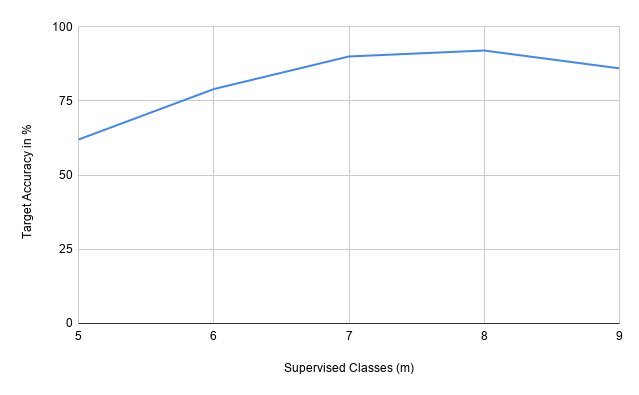
\includegraphics[width=0.8\textwidth]{abbildungen/mixedResults.png}
  \caption{Results of the experiments with the DSN': Target accuracy of the DSN' with all losses activated when trained $m$ supervised classes from $S$ and $M$.}
  \label{dia:mixedDSN}
\end{figure}

\begin{figure}[tbh]
  \centering
    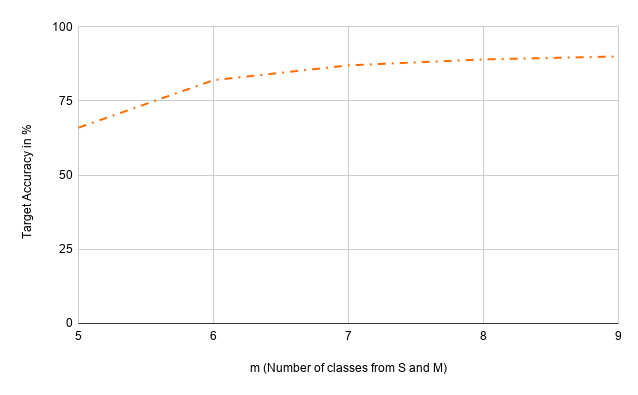
\includegraphics[width=0.8\textwidth]{abbildungen/mixeddaResults.png}
    \caption{Results of the experiments with the DSN' sim: Target Accuracy of the DSN' with only similarity loss activated trained on $m$ supervised classes from $S$ and $M$. This setup has a similar architecture to DANN.}
  \label{dia:mixedDA}
\end{figure}

\paragraph*{Discussion} Our results confirm the observation made in \cite{domainMixture} regarding the quasi constant performance of the model when it uses domain adaptation on the mixed domains. This also proves the architecture's ability to extract domain-free representations with which the classifier can train effectively even when multiple domains are present and the domains are incomplete.

However, a remarkable notice is, in our setup, the performance gap between training on a domain with 5 supervised classes from each domain and training with 6 classes per domain. On one hand, this should not be surprising since more supervised data offers more information and having more supervised classes resembles traditional machine learning that needs no domain adaptation. On the other hand, we have seen that the model can cope well with missing domain-class representation for $m \geqslant 6$ but performs unproportionally worse when $m=5$. After considering the differences between the architecture and the setups, we propose these possibilities to answer for this behavior:

\paragraph*{Overfitting} As we know, learning repeatedly on the same data for too much could make the network memorizes the training and therefore inhibits its ability to generalize the task to the unknown data. As we chose to train the network with an equal number of update step for all the number of classes $m$ within the same setup, the variation with only 5 supervised domains would offer the least amount of data among them and could therefore cause overfitting. To check this possibility, we evaluate the model at earlier training stages, i.e., as less learning steps have been made. The earlier performances on these steps also show no significant signs of overfitting, they perform partly equivalent and partly worse than the end results shown above. Therefore, the evidences seem not to point to overfitting as the cause of this behavior. 

\paragraph*{Randomly Assembled Batches} After negating the overfitting as the cause of this performance gap, we look for a difference between our experiments and those in \cite{domainMixture}. A difference we regard as a possible cause is how we generate batches for the gradient descent. In \cite{domainMixture}, they explicitly generate batches with half supervised samples and half unsupervised. Hence, the classifier has something to train on in every steps equally to the domain classifier can learn about the domains. In our experiments, we generate the batches by randomly choose the data in the mixed domains. It is therefore possible that the classifier did not trained equally well in each step and might be still underdeveloped or developed in the sub-optimal way. Ideally, the experiments should be repeated with similarly generated batches to observe the results. We consider this to be an open question requiring further studies. 

\paragraph*{Reaction of the DSN to lack of Overlapping Supervised Classes} Another speculation to explain this behavior is that the DSN reacts differently on the extra overlapping domain-class combinations offered in cases of $m \geqslant 6$. We call this a speculation because there is no obvious reason regarding the architecture. Only the similarity loss activated, the DSN actually includes the same mechanisms as the DANN in that it learns adversarially with the gradient reversal layer and the classifier is feed only with representations created from the shared encoders. A confusion matrix similar to that in \cite{domainMixture} could be calculated to see what kind of false predictions were being made. Whether it uses the different domain to make assumption about the classes that one domain could not include those classes it only has seen in another domain in the training. This possibility needs to be further investigated to understand this behavior better. \\

\begin{figure}[tbh]
  \centering
    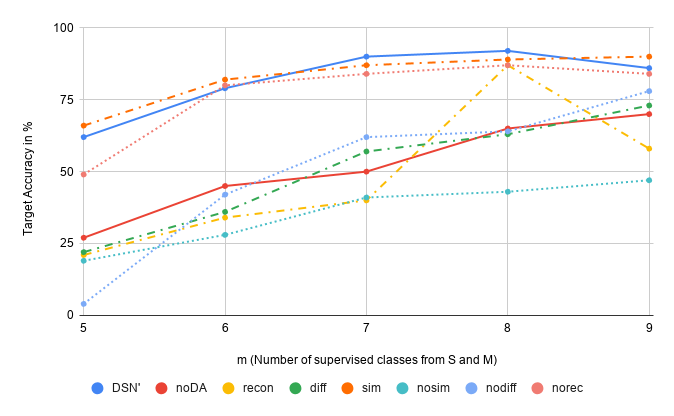
\includegraphics[width=0.8\textwidth]{abbildungen/allDSNResults.png}
    \caption{Results of all the DSN' setups: Target Accuracy of all the DSN' variations experimented on the complete domain mixture scenario with different mixture combinations out of $m$ supervised classes from both $S$ and $M$.}
  \label{fig:allDSNResults}
\end{figure}

To see the impacts of each different losses on the performance of the DSN, the experiments were also carried with different loss combinations. All the combinations tested and their abbreviation used in this thesis are listed in Table \ref{tb:lossCombinations} in Section \ref{sec:exSetups}. The target accuracies of all the settings are plotted in Figure \ref{fig:allDSNResults}.

The worst average performance is delivered when the similarity loss is deactivated, as seen in the 'nosim' case. The DSN' makes overall even more inaccurate prediction with this loss combination than without any loss activated - the no domain adaptation 'noDA' case. This may result from the constraints put on the networks through other activated losses while the classifier already has to train on the domain-contaminated representations - the similarity loss responsible for the domain-independent shared representations is deactivated and the other losses further complicate the optimization problem. An evidence supporting this argument is that other setups such as 'recon' and 'diff' which are also trained without the similarity loss perform better quasi overall better with only one other loss activated. 

Another interesting point is the peak performance at $m = 8$ of the 'recon' setup with only reconstruction loss activated. At $m = 8$, the DSN' with this setup has an almost constant target accuracy of 86\%, even better than at $m = 9$. It is possible that these good results could be only straying outliers. With the existing data, this possibility cannot be eliminated, further runs with this setup should be executed again. A conclusion that $m = 8$ is the 'golden spot' of this setup cannot be made yet since there is no supporting argument. 

It is also clear to see that the similarity loss has the most impact on the target accuracy of the setups. All the combinations with this loss deactivated perform significantly worse than those with this loss activated. The differences between these combinations seem to decrease with more supervised data. The strong dependence of the performance on the similarity loss is understandable because the similarity loss is the key to creating domain-irrelevant representations on which the classifier can train to perform domain transfer at its best according to a theory of domain adaptation. Other losses, the reconstruction loss and the difference loss, seem to be complementary to the similarity loss.

On the contrary, deactivating only reconstruction loss appears to affect the performance of the DSN' only minimally. This setup, referred to as 'norec', performs only slightly worse than the setup with all losses activated (DSN') and with only similarity loss activated (sim). 

The last remarkable insight seen in the graph is the significantly low accuracy of only 4\% of the 'nodiff' DSN' at $m = 5$. As mentioned above, removing the similarity highly affects the performance. However, the average performance of this particular setup is significantly low. In many runs with this setup, the accuracy is almost 0 whereas some of them even reach 30\%. Since $m = 5$ offers less information, it is imaginable that overfitting could be the cause. A look on the recorded target accuracy over the training phase, however, indicates no clear signs of overfitting or anomaly in the training. The target accuracy seems to normally converge against 0. This high variance in the performance among the same setup and the significantly low performance at $m=5$ should be studied further. For this, a confusion matrix, for instance, could also offer useful information on this behavior similar to the aforementioned problem of the performance gap.

Generally, these bad results and unstable results, i.e., big differences in performance between runs, can also be observed in many setups with $m = 5$ or $m = 6$ . The model apparently trains more stably and more effectively with more supervised data. 

 There are more potential works to be done which unfortunately cannot be included into this thesis due to time restriction. For example, the investigation of the performance gap, the significantly low performance and the unstable performances between runs should be carried further. Further studies on the influences of different losses on the performance of the network could be useful in designing further architectures inspired from these different parts of the DSN. 

